%!tex program = lualatex
\documentclass[answers]{exam}
\usepackage{ctex}
\usepackage{graphicx}
\usepackage[margin=2cm]{geometry}
\usepackage{amsmath, amssymb}
\usepackage{csquotes}
\usepackage{tikz, pgfplots}
\usetikzlibrary{
	angles,
	backgrounds,
	calc,
	decorations.pathmorphing,
	decorations.pathreplacing,
	decorations.text,
	intersections,
	patterns,
	quotes,
	shapes,
	shapes.symbols,
}
\pagestyle{empty}
\newcounter{xcord}
\newcounter{ycord}
\newcounter{total}
\renewcommand{\labelenumi}{\textbf{\ifnum\value{enumi}<10 0\fi\arabic{enumi})}}

\pgfplotsset{compat=1.18}

\CorrectChoiceEmphasis{\color{blue!70!green}\bfseries}
\renewcommand{\solutiontitle}{\textbf{解:}}

\usepackage{array, tabularx}
\newcolumntype{C}{>{\centering\arraybackslash}X}
\newcolumntype{B}{>{\centering\bfseries\arraybackslash}X}
\catcode`\幺=0

\usepackage{tkz-euclide}

\begin{document}
\begin{center}
	\textbf{1997年普通高等学校招生考试(全国卷)}

	\textbf{\Large 理科数学}
\end{center}
\begin{questions}
	\question 设集合$M=\{x|0 \leqslant x < 2\}$,集合$N=\{x|x^2 - 2x - 3 <0\}$,集合$M\cap N=$ \hfill (\hspace{2cm})
	\begin{oneparchoices}
		\choice $\{x|0\leqslant x < 1\}$
		\CorrectChoice $\{x|0\leqslant x < 2\}$
		\choice $\{x|0\leqslant x \leqslant 1\}$
		\choice $\{x|0\leqslant x \leqslant 2\}$
	\end{oneparchoices}

	\begin{solution}
		集合$N=\{x|-1 < x < 3\}$,两个集合的范围如下图所示:

		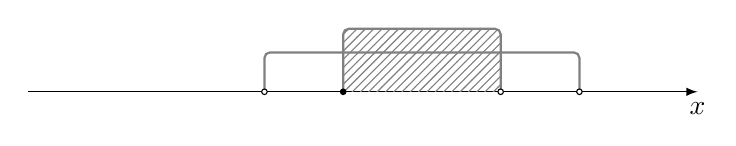
\begin{tikzpicture}
			\tkzInit[xmin=-4, xmax=4]
			\tkzDrawX

			\draw[rounded corners=2pt, thick, black!50] (-1,0) |- (3,.5) -- (3,0);
			\draw[black!50, thick, pattern=north east lines,pattern color=black!50, rounded corners=2pt] (0,0) |- (2,.8) -- (2,0);
			\draw [fill=white](-1,0) circle (1pt);
			\draw [fill=white](3,0) circle (1pt);
			\draw [fill=black](0,0) circle (1pt);
			\draw [fill=white](2,0) circle (1pt);
		\end{tikzpicture}
	\end{solution}

	\question 如果直线$ax+2y+2=0$与直线$3x-y-2=0$平行,那么系数$a=$ \hfs

	\begin{oneparchoices}
		\choice $-3$
		\CorrectChoice $-6$
		\choice $-\dfrac32$
		\choice $\dfrac23$
	\end{oneparchoices}

	\begin{solution}
		两条直线平行则其斜率相等,可得:
		\begin{equation*}
			-\frac{a}{2} = 3
		\end{equation*}
		所以答案为$a=-6$
	\end{solution}

	\question 函数$y=\tan \left( \dfrac12x - \dfrac{\pi}{3} \right)$在一个周期内的图像是 \hfs

	\begin{oneparchoices}
		\pgfplotsset{
			xlabel={$x$},
			ylabel={$y$},
			x label style={at={(current axis.right of origin)}, anchor=north},
			axis lines=center,
			samples=100,
			ticks=none
		}
		\CorrectChoice
		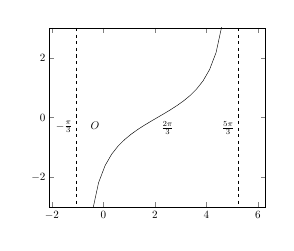
\begin{tikzpicture}[scale=.4]
			\begin{axis}[
					xmin = {-2/3*pi},
					xmax = {2*pi},
					ymin = -3,
					ymax = 3,
				]
				\addplot[domain={-1/3*pi+0.1}:{5/3*pi-0.1}]{tan(deg(1/2*x - pi/3))};
				\draw[dashed] (-pi/3,3) -- (-pi/3, -3);
				\draw[dashed] (pi*5/3,3) -- (pi*5/3, -3);
				\node[below left] at (-pi/3, 0) {$-\frac{\pi}{3}$};
				\node[below right] at (2*pi/3, 0) {$\frac{2\pi}{3}$};
				\node[below left] at (5*pi/3, 0) {$\frac{5\pi}{3}$};
				\node[below left] at (0,0) {$O$};
			\end{axis}
		\end{tikzpicture}
		\choice
		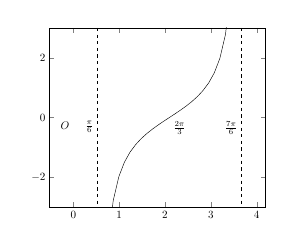
\begin{tikzpicture}[scale=.4]
			\begin{axis}[
					xmin = {-1/6*pi},
					xmax = {8/6*pi},
					ymin = -3,
					ymax = 3,
				]
				\addplot[domain={1/6*pi+0.1}:{7/6*pi-0.1}]{tan(deg(x - 2/3*pi))};
				\draw[dashed] (pi/6,3) -- (pi/6, -3);
				\draw[dashed] (pi*7/6,3) -- (pi*7/6, -3);
				\node[below left] at (pi/6, 0) {$\frac{\pi}{6}$};
				\node[below right] at (2*pi/3, 0) {$\frac{2\pi}{3}$};
				\node[below left] at (7*pi/6, 0) {$\frac{7\pi}{6}$};
				\node[below left] at (0,0) {$O$};
			\end{axis}
		\end{tikzpicture}
		\choice
		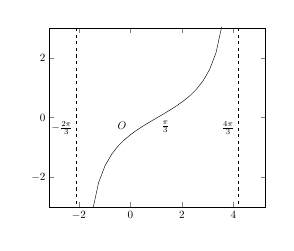
\begin{tikzpicture}[scale=.4]
			\begin{axis}[
					xmin = {-pi},
					xmax = {5/3*pi},
					ymin = -3,
					ymax = 3,
				]
				\addplot[domain={-2/3*pi+0.1}:{4/3*pi-0.1}]{tan(deg(1/2*x - pi/6))};
				\draw[dashed] (-pi*2/3,3) -- (-pi*2/3, -3);
				\draw[dashed] (pi*4/3,3) -- (pi*4/3, -3);
				\node[below left] at (-pi*2/3, 0) {$-\frac{2\pi}{3}$};
				\node[below right] at (pi/3, 0) {$\frac{\pi}{3}$};
				\node[below left] at (4*pi/3, 0) {$\frac{4\pi}{3}$};
				\node[below left] at (0,0) {$O$};
			\end{axis}
		\end{tikzpicture}
		\choice
		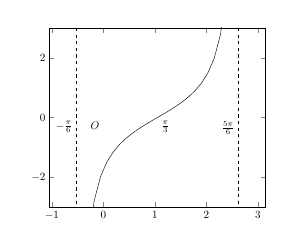
\begin{tikzpicture}[scale=.4]
			\begin{axis}[
					xmin = {-1/3*pi},
					xmax = {pi},
					ymin = -3,
					ymax = 3,
				]
				\addplot[domain={-1/6*pi+0.1}:{5/6*pi-0.1}]{tan(deg(x - 1/3*pi))};
				\draw[dashed] (-pi/6,3) -- (-pi/6, -3);
				\draw[dashed] (pi*5/6,3) -- (pi*5/6, -3);
				\node[below left] at (-pi/6, 0) {$-\frac{\pi}{6}$};
				\node[below right] at (pi/3, 0) {$\frac{\pi}{3}$};
				\node[below left] at (5*pi/6, 0) {$\frac{5\pi}{6}$};
				\node[below left] at (0,0) {$O$};
			\end{axis}
		\end{tikzpicture}
	\end{oneparchoices}
	\begin{solution}
		$\tan{x}$的周期是$\pi$,所以$\tan{\frac12{x}}$的周期应该为$2\pi$.因此排除B和D.
		$\tan(\frac12\cdot\frac{\pi}{3}-\frac{\pi}{3}) \neq 0$,因此选A.
	\end{solution}
	\question
	已知三棱锥$D-ABC$的三个侧面与底面全等,且$AB=AC=\sqrt{3}$,$BC=2$,则以$BC$为棱,以面$BCD$与面$BCA$为面的二面角的大小是
	\hfs

	\begin{oneparchoices}
		\choice $\arccos\dfrac{\sqrt{3}}{3}$
		\choice $\arccos\dfrac{1}{3}$
		\CorrectChoice $\dfrac{\pi}{2}$
		\choice $\dfrac{2\pi}{3}$
	\end{oneparchoices}

	\begin{solution}

		\tdplotsetmaincoords{20}{120}
		\begin{center}
			\begin{tikzpicture}[tdplot_main_coords, baseline=(current bounding box.north)]
				\coordinate(A) at ({sqrt(2)}, 0);
				\coordinate(B) at (0,1);
				\coordinate(C) at (0,-1);
				\coordinate(D) at (0,0,{sqrt(2)});

				\draw(A)node[below]{$A$} -- (B)node[below]{$B$};
				\draw[dashed](B)-- (C)node[above]{$C$};
				\draw(C)-- (A);
				\draw(D)node[above]{$D$} -- (A);
				\draw(D) -- (B);
				\draw(D) -- (C);

				\draw[blue, dashed](A) -- (0,0)node[below right]{$O$} -- (D);
			\end{tikzpicture}
		\end{center}

		取$BC$的中点为$O$,连接$AO$和$DO$.
		因为$AC=AB$,所以有$AO\perp BC$.因为$\triangle{BCD}\cong\triangle{BCA}$,所以也有$DO\perp
			BC$.计算可得$AO=DO=\sqrt{2}$.另外有$AD=2$.可以看出有$AO^2 + DO^2 =
			AD^2$,所以$\triangle{AOD}$是直角三角形,即二面角为$\ang{90}$.
	\end{solution}

	\question 函数$y=\sin \left( \dfrac{\pi}{3} - 2x \right) + \cos2x$的最小正周期是 \hfs

	\begin{oneparchoices}
		\choice $\dfrac{\pi}{2}$
		\CorrectChoice $\pi$
		\choice $2\pi$
		\choice $\dfrac{2\pi}{3}$
	\end{oneparchoices}

	\begin{solution}
		因为$\sin \left( \dfrac{\pi}{3} -2x \right)$与$\cos2x$的周期均为$\pi$,所以函数的最小正周期也为$\pi$.
	\end{solution}

	\question 满足$\arccos(1-x) \geqslant \arccos{x}$的取值范围是 \hfs

	\begin{oneparchoices}
		\choice $\left[-1, -\dfrac12\right]$
		\choice $\left[-\dfrac12, 0\right]$
		\choice $\left[0, \dfrac12\right]$
		\CorrectChoice $\left[\dfrac12, 1\right]$
	\end{oneparchoices}

	\begin{solution}
		因为$\arccos$的定义域是$[-1,1]$,所以排队选项A和B.

		$\arccos(0) = \frac{\pi}{2}, \arccos(1-0)=0$,所以C也可以排除.答案为D.
	\end{solution}

	\question 将$y=2^x$的图像\underline{\hspace{.5cm}},再作关于直线$y=x$对称的图像,可得到函数$y=\log_2(x+1)$的图像. \hfs

	\begin{oneparchoices}
		\choice 先向左平移$1$个单位
		\choice 先向右平移$1$个单位
		\choice 先向上平移$1$个单位
		\CorrectChoice 先向下平移$1$个单位
	\end{oneparchoices}

	\begin{solution}
		点$(0,0)$在直线$y=x$上,并且也在函数$y=\log_2(x+1)$上,所以应该也在$y=2^x$平移后的图像上,可以得到平移后的图像为$y=2^x
		- 1$才能满足点$(0,0)$在图像上.
	\end{solution}

\end{questions}
\end{document}
